%\section*{Project Description}
\section{Introduction and Goals}
Anthropogenic pressure and other natural causes have resulted in
severe disruption of the global ecosystems in recent years, including
climate change with extreme weather events, change (loss) of
biodiversity, and invasion of non-native flora and fauna. The deforestation of
rainforests and degradation of natural habitats is happening faster
than efforts to study and understand the impact of these environmental
insults.  Beyond undesired changes, recent years have also seen an increase in experimental genetics
experiments that could radically change the
population distribution in an environment. For example, the Target Malaria project
is a \$75M effort using CRISPR gene drives to genetically modify, and
eliminate mosquitoes (\emph{Anopheles}), and could be deployed in
Africa within 2 years\cite{TargetMalaria}, but its impact on the local
biogeography is completely unknown.  Similar gene drives are being
organized to eliminate Avian malarial parasite carrying mosquitoes
from Hawaii\cite{Liao2017}, and Rodents from New Zealand\cite{Owens2017}.  

The ability
to quickly and inexpensively sample the taxonomic diversity in an
environment in real time is critical in this era of rapid climate and biodiversity
changes, and for the ethical
conduct of these directed evolution experiments in nature\cite{Oye2014}. Indeed, such methods are specifically important for organisms such as arthropods\cite{Beng2016} and small plants, which are among the most abundant and diverse
non-microbial organisms on Earth but lack large-scale descriptions of
biogeography and richness. However, large
cataloging surveys remain sparse. At least some of this discrepancy
can be attributed to the high cost of sorting and identifying samples
from large sampling collections. 

%With the advent of next generation sequencing methods, 
The molecular
technique of choice for measuring biodiversity is
(meta)barcoding\cite{Hebert2003,Savolainen2005,Taberlet2012}, which
involves DNA sequencing of taxonomically informative and
group-specific markers (e.g., mtDNA COI~\cite{Seifert2007,Hebert2003}
and 12S/16S \cite{Vences2005} for animals, plastid genes like trnl and
matK~\cite{Hollingsworth2009} for plants, and ITS~\cite{Schoch2012}
for fungi) that are variable enough for taxonomic identification, but
have flanking regions that are sufficiently conserved to allow for PCR
amplification using universal primers. Barcoding is used to
taxonomically identify species or in the case of meta-barcoding to
deconstruct the species composition of complex samples.  
%Barcode markers have also been used  in phylogenetics\cite{Hedin2001,Taylor2017}.  
Accurate
barcoding crucially depends on the coverage of the reference database and the method used
to search the  database~\cite{Taberlet2012}.
Computational methods have been developed for finding the closest match in a reference
dataset of markers (e.g., TaxI\cite{taxl}), and for placement of a
query into existing marker trees\cite{epa,pplacer}. The reference databases for these studies consist of traditional barcode regions, such as COI in the Barcode of
Life Data System\cite{BOLD}.  

The traditional barcoding
pipeline has several drawbacks.  PCR for marker gene amplification requires relatively high-quality DNA and thus cannot be applied to samples in which the DNA is heavily fragmented.  Moreover,
since barcodes are short regions, their phylogenetic signal is limited\cite{Hickerson2006b}.  For
example, 896 of the 4,174 species of wasps could not be
distinguished from other species using COI barcodes\cite{Quicke2012}.
While low costs have kept PCR-based pipelines attractive, falling
costs of shotgun sequencing have now made it possible to shotgun
sequence 1-2Gb of a reference specimen sample for 
$\le\$50$, inclusive of sample preparation and labor costs.
Therefore, researchers have proposed low-pass sequencing (\emph{genome-skimming}) as
a viable approach to
barcoding\cite{Coissac2016}. These approaches identify chloroplast/mtDNA marker genes in genomes by mapping to a reference library or \emph{de novo} assembly\cite{Liu2013}. 
Large 
databases (e.g., through PhyloAlps~\cite{PhyloAlps} and
 NorBol~\cite{NorBol} projects) are using genome-skimming to mine marker genes. 
Our Danish collaborators ({\bf letter: Gilbert}) have developed a similar genome-skimming project, DNAmark~\cite{DNAmark}. However, they realized that {\em accurate} assembly of organelle and
marker regions from genome-skims is non-trivial, and the approach discards the vast majority of the reads and is thus
wasteful.  Therefore, they posed an interesting methodological
question: \emph{can the unassembled data be used ``as-is'' for barcoding, saving on the labor-intensive task of mtDNA assembly and using all available genomic information?}

Motivated by this question, we consider the alternative approach where low coverage genome-skims are used both to create the reference library and the query dataset.
%Here, we treat genome-skims simply as low-coverage ``bags of reads'',both for the orphan \emph{query}, and for a \emph{library} of(non-assembled) \emph{reference} genome-skims obtained for a collection of known species. 
We propose the development of computational and statistical tools to address the
following key questions (Figure~\ref{fig:overview}):
\begin{packed_desc}
%[label={\bf A\arabic*}:]
\item [Aim 1:] 
\item [Aim 2:] 
\item [Aim 3:] 
\end{packed_desc}
\begin{figure}
\centering
  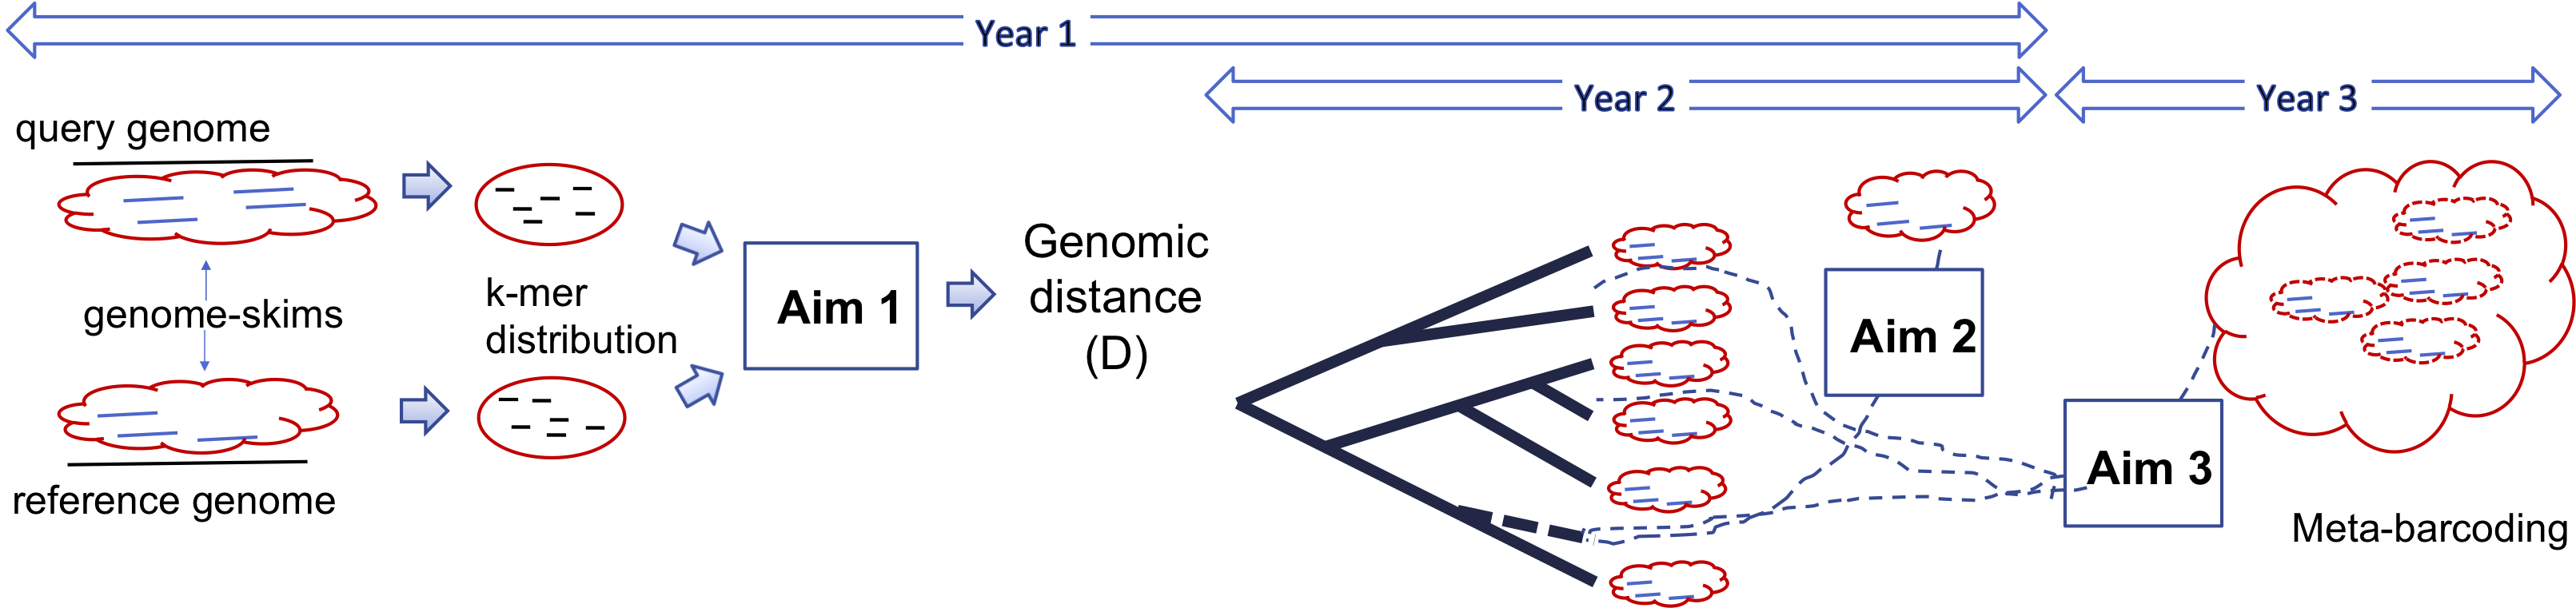
\includegraphics[width=1\textwidth]{fig/Overview.png}
\vspace{-20pt}\caption{{\bf Overview of the scientific aims.}}
  \label{fig:overview}
\end{figure}
As this is a \emph{short}, exploratory, proposal budgeting for four graduate student years, we will address Aims 1 (Year 1) and Aim 2 (Years 1 and 2) thoroughly and will perform exploratory empirical and theoretical work on Aim 3 (Year 3) in preparation for a larger, collaborative proposal.

\section{Broader Impacts}

The proposed activities have broad impact because some of the poorest and under-developed places have most of the
remaining bio-diversity in the world. The loss of this bio-diversity can
have severe and lasting impact on all people, including in the
U.S.A. However, even with dramatically falling costs, genomic
sequencing technologies have not penetrated these communities. We will use the grant period to reach out to scientists and build collaborations that start to catalog genome-skims, similar to
barcoding efforts such as the Consortium for the Barcode of Life.  
We will collaborate with Dr. Thomas Gilbert, leader of the center for GeoGenetics at the Natural History
Museum of Denmark on developing metabarcoding. 
We will also
initiate a collaboration with Dr. Ethan Bier (UC San Diego, and Tata
Institute of Genomics and society) who is developing CRISPR based
technologies to change \emph{Anopheles} population composition in some
locations in India with the goal of eliminating malaria. We will use
these initial studies to develop inexpensive protocols that will allow anyone in the world to gather genome-skims that can be
analyzed by our publicly available tools.  
Beyond these, 
we will make outreach efforts: i)
train STAR undergraduate students, recruited from both biology and CS;
ii) the annual Evolution meeting includes an outreach program promoting the understanding of computational technique; we will participate in Year 3 and use barcoding using genome-skims as an example  to promote computational understanding among biology undergraduates;
iv) we will hold local seminars to increase awareness of the impact of rapid environmental changes on
ecology and the role of 
computational genomics  in 
alleviating them.
%Taken together, the impact  of our proposed work exceeds the impact of the proposed algorithmic work.




\paragraph{Preliminary Results.}




\paragraph{{\large Challenges and proposed goals}.}


\paragraph{A1.3 Contamination.}
A major issue that we have so far ignored is 
the possibility that external DNA originating from parasites, diet, fungi, bacteria, and human contamination may be mixed 
with a supposedly single-species genome-skim.
The presence of such external DNA can negatively impact the estimated distance. 
%We plan to address this shortcoming in several ways.
%\begin{enumerate*}[itemjoin={.\quad},label=\roman*)]
%\item 
We will perform extensive tests
to quantify the robustness of \skmer\ to 
external DNA by manually injecting
fungal, bacterial, and human contamination.
Moreover, so far, we have tested \skmer\  only on simulated genome-skims. 
We plan to collaborate with our DNAmark colleagues
to test \skmer\ on real genome-skims from known species. 

To improve \skmer\ in the presence of external DNA,
several approaches can be considered.
For genome-skims in the reference library,
we can simply search a database using tools like BLAST~\cite{blast}, USearch\cite{usearch}, or Bowtie~\cite{Langmead2012a}, or faster k-mer based methods like Kraken~\cite{Kraken}  to find and eliminate bacterial or fungal contamination.
Note that the cost of preprocessing will be amortized over many searches.
%Reads with significant hits to species other than the taxonomic group of interest can be simply eliminated from the
%reference library.

For query sequences, even a fast classification tool like Kraken run on all reads \textit{may} prove too slow.
But note that we don't need identities of contaminants.
 \emph{Given a query genome-skim, and a large `contaminant database' of genome skims from prokaryotes and fungi, we will develop super-fast algorithms for filtering contamination}.
We will test membership queries using Bloom filters representing the union of k-mers in all contaminant sequences. Consider a bit-vector $B$ of size $m$, where each of $n$ k-mers from a contaminant set is hashed using $h$ bits. Then, the probability of a non-contaminant k-mer being hashed to $B$ by chance, $p \le (1-e^{-\frac{hn}{m}})^h$. We will denote a read as a contaminant if a fraction $\theta$ of its k-mers are hashed to $B$. For small $p$, the probability of mis-classifying a read as a contaminant is bounded using Chernoff's bound to be $\le\text{exp}(-\ell(\theta-p)^2)$.
 Adjusting $\theta$, we 
 can also detect contamination from species
 {\em close to} but not identical to those
 in our database. 
Thus, Bloom filter may provide a super-fast way of eliminating all contaminant reads.

For even higher speeds, {\em we will develop algorithmic strategies to compute the true distance  without eliminating contaminants}. 
For a query genome-skim with a mix
of $k$-mers from the real species  ($A$)
and those from contaminants ($C$), and reference skim $B$,
let $J'$ be the Jaccard computed
without filtering.
We can estimate the fraction of contamination $w=\frac{|A|}{|A\cup C|}\approx\frac{|A|}{|A|+|C|}$
% We will compute the Jaccard 
% index between a genome-skim of a pure 
% reference species and a mix of $w$\% reads from a 
% main query species and $(100-w)$\% reads from several contaminant species.
by running Kraken or
the Bloom filter  on a small subset of reads.
We expect contaminants to have very low similarity to the main query species (e.g., fungal DNA in an insect query). Thus, 
their contribution to the shared $k$-mer set is negligible (i.e.,
$|A\cap C|\approx |B\cap C|\approx 0$). 
Note also that $|A\cup B \cup C|$ and $|A\cup C|$ can be easily computed using JellyFish.
Then, we can derive
the corrected $J$:
\vspace{-6pt}
\begin{small}
$$J=\frac{|A\cap B|}{|A\cup B|}=\frac{|A\cap B|/{|A\cup B \cup C|}}{|A\cup B|/|A\cup B \cup C|}=\frac{J'}{1-\frac{|C|}{|A\cup B \cup C|}}=\frac{J'}{1-(1-w)\frac{|A\cup C|}{|A\cup B \cup C|}}\; .
\vspace{-3pt}
$$
\end{small}
Thus, we can use Equation~\ref{eqn:distance_estimate_penalized} with
this contamination-corrected estimate of $J$.
%\end{enumerate*}
This way of handling contamination 
is essentially a simpler case of meta-barcoding (Aim 3)
because we  assume {\em a priori} that contaminants
are distant from the main query species
and do not seek their identity. 

%\paragraph{A1.4 Testing on real data.}


\vspace{-5pt}
\section{Intellectual merit}
\vspace{-5pt}
The proposed research creates a novel paradigm for measuring
biodiversity. If successful, the activities will allow us to sample
genomes of multiple organisms for a fraction of the current costs of
labor and genome sequencing required for other approaches. The
proposal uses a number of novel algorithmic and statistical ideas to
correctly estimate genomic distance based on
genome-skims. Specifically, it will be the first systematic analysis
of how close we can get to computing the genomic distance using only a
small and random fraction of an individual's genome. The proposed
methods can easily be extended to other vexing problems such as the
identification of phylogenetic placement of a previously unknown
organism, provenance of a museum animal, 
sibling analyses, and possibly forensic
science. The investigators have a strong history of prior research in
related fields, but have complementary expertise. Lead PI Mirarab is
an expert in evolution and phylogeny reconstruction of organisms and
helped reconstruct the state of the art in avian\cite{avian} and plant~\cite{1kp-pilot}
phylogeny, has developed highly
used tools for phylogeny inference~\cite{astral,astral2} and
metagenomics\cite{sepp,tipp}. PI
Bafna has expertise in genomics, and the use of novel techniques for
analyzing complex structural variation\cite{Turner2017} as well as the
development of new sequencing technologies and computational tools for
analyzing the resulting data\cite{Chu2017,Edge2017,Patel2014}. He also has expertise in
population genetics, and the impact of environment (selection
processes) in shaping the population genetic variation landscape\cite{Ronen2014,Ronen2015}.



%\section{Broader Impacts of the Proposed Work}


\vspace{-5pt}
\section{Results from Prior NSF Support}
\vspace{-5pt}

\noindent
\emph{\underline{Bafna}}: NSF-III (1318386) ``Algorithms for decoding complex patterns of genomic variation'' (\$500K, 9/01/13-8/31/17).  
{\bf Intellectual Merit:} Multiple publications resulted from this grant\cite{Lo2013,Ronen2013,Zhou2013,Lo2013b,Patel2014,Udpa2014,Kramer2014,Kinsella2014,Ronen2014,
Chen2015,
Zakov2015,Ronen2015,Flannery2015,Beyter2016,Patel2016,Stobdan2015,
Azad2016, Ronen2016, Edge2017, Iranmehr2017, Azad2017, Stobdan2017}, focused on exploiting the allele frequency spectrum for identifying regions under selection, experimental evolution, haplotype assembly, and decoding of complex structural variation. {\bf Broader Impacts:} include software tools, CLEAR for analyzing experimental evolution\cite{Iranmehr2017}, InPhaDel\cite{Patel2016} and Hapcut2\cite{Edge2017} for haplotyping, and PreCIOSS for identifying carriers of a selective sweep\cite{Ronen2015}.

\noindent
\emph{\underline{Mirarab}}: III (1565862) ``Using Genomic Context to Understand Evolutionary Histories of Individual Genes'' (\$175,000, 7/1/2016--6/30/2018). {\bf Intellectual Merit:} 
Several publications have results from the grant~\cite{distique,MVroot,Shekhar2017,insects,astral3,Mai2017,dual-birth}.
{\bf Broader Impacts:} 
include several publicly available software
tools: DISTIQUE~\cite{distique},
MV Rooting~\cite{MVroot}, ASTRAL-3~\cite{astral3}, and TreeShrink~\cite{Mai2017}.
All tools are available at
{\tt http://eceweb.ucsd.edu/~smirarab/software.html}.
%   \url{https://github.com/smirarab/},
%   \url{https://github.com/uym2/},
%     \url{https://github.com/uym2/}, and
%     \url{https://github.com/niemasd}.
%   \url{https://github.com/smirarab/ASTRAL},
%   \url{https://github.com/uym2/MinVar-Rooting},
%   \url{https://github.com/uym2/TreeShrink},
%     \url{https://github.com/esayyari/DISTIQUE},
%   \url{https://github.com/niemasd/Dual-Birth-Model}
We have also created benchmark datasets
for the community to use:
%   \url{https://uym2.github.io/MinVar-Rooting/},
%   \url{https://esayyari.github.io/InsectsData},
 {\tt https://sites.google.com/eng.ucsd.edu/datasets/}.
 We also mentored three undergraduate students, one through the STAR program, through this project.
